\section{FPGA}

Field Programmable Gate Arrays (FPGAs) are integrated circuits
containing gate matrix which can be programmed by the user
"in the field" without using expensive equipment.

An FPGA contains a set of programmable logic gates and rich interconnect
resources, making it possible to implement complex digital circuits.

The majority of FPGAs are based on SRAM. (Static RAM).

FPGA mainly consists of three types of modules.
I/O blocks, switch matrix/interconnection wires and configurable
logic blocks (clb).

The I/O blocks are used to interface with the external world.
This could be a sensor, a display or a communication device.

Configurable logic blocks consists of look-up tables (LUTs),
flip flops and multiplexers.
A LUT is a memory unit that can store data and output the stored data.
The part that is programmed with VHDL is in the LUTs.


\begin{center}
	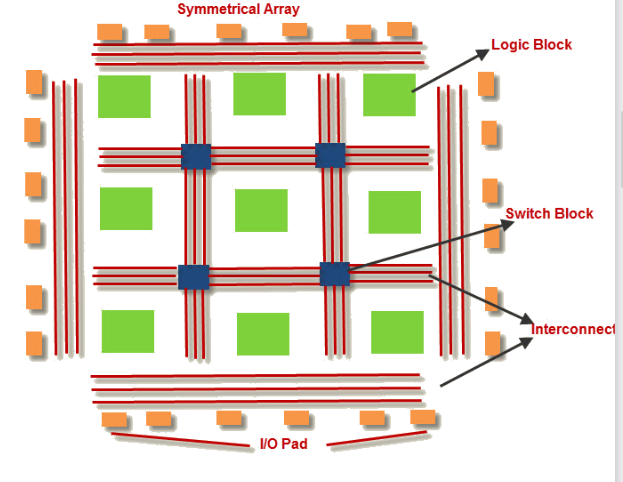
\includegraphics[width=0.6\textwidth]{images/fpga.png}
\end{center}


\begin{center}
	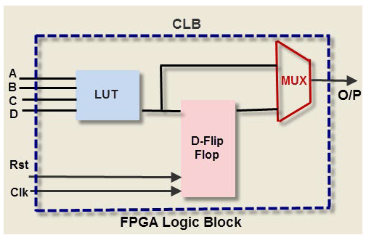
\includegraphics[width=0.4\textwidth]{images/clb.png}
\end{center}


\textbf{SRAM-based FPGAs}

It stores logic cells configuration data in the static memory.
Since SRAM is volatile, the FPGAs must be programmed upon start.
There are two basic modes of programming:

Master mode: The FPGA is programmed by an external device such as an
external flash memory chip.
Slave mode: The FPGA is configured by an external master device,
such as a processor.

SRAM based FPGAs with an internal flash memory:
It contains internal flash memory blocks, thus eliminating the need to have
an external non-volatile memory. It uses flash only during startup to load
data to the SRAM configuration cells.


\textbf{Programmable switch FPGAs}

It uses flash as a primary resource for configuration storage,
and doesn't require SRAM.

Switch is a floating-gate transistor that can be turned off by
injecting charge onto its floating gate.
It has a limited number of reprogramming, but is more secure
than SRAM-FPGA.


\textbf{Fuse-based FPGA}

One time program FPGA.
The fuse makes or breaks link between two wires.
Making it more secure than SRAM (no load from an external device)
In high radiation environments, radiation events can cause SRAM,
that contains the program, to change state but not in fused FPGA.

\textbf{Programmable switch matrix}

All internal connections are composed of metal segments with
programmable switching points and switching matrices to
implement the desired routing.



\textbf{Design flow}

VHDL files. Goes to synthesis, then to implementation on the board
and at last configuration where the FPGA is tested.

After the synthesis where the code is translated into logic gates,
the logic gates are mapped into lut's on the logic blocks. After
this placing routing is done, where the interconnections are
wired using the switch blocks.


Once a design is implemented, the synthesis tool generates a file that
the FPGA can understand. This file is called a bit stream.
The bit file can be downloaded directly to the FPGA, or can be converted
into a PROM file which stores the programming information.


\subsection{CPLD}

Complex Programmable Logic Devices (CPLDs) are similar to FPGAs,
but they have fewer logic blocks and more interconnect.

Logic block signals only connect to the neighboring logic blocks.
Nonvolatile logic cells (based on EEPROM Flash), on when powered.

CPLDs implement sum of product style logic not LUT as in FPGA.
They are good for simple applications and cheaper.
